\documentclass{beamer}
\title{EDET Chipset Upgrades}
\author{Kennedy Caisley}
\institute{University of Bonn}
\date{27 March, 2024}

\begin{document}
\beamertemplatenavigationsymbolsempty

\frame{\titlepage}


\begin{frame}
    \frametitle{Application Basics [Epp 2016 VERTEX]}
    \begin{itemize}
    \item Time resolution $10^{-3}$ - $10^{-6}$, i.e. structural changes in biology
    \item $60\mu m$ pitch, $50\mu m$ thickness, signal mostly in-pixel
    \item 300 kEV $e^-$ source $\rightarrow$ $\approx$8000 e-h pairs in $50\mu m$ Si
    \item 100+ primaries in most pixels ($>1000ke^-$ signal); only a couple under target

    \end{itemize}
\end{frame}

\begin{frame}
    \frametitle{Detector Characteristics [Predikaka 2022 Thesis/NIMA]}
    \begin{figure}
    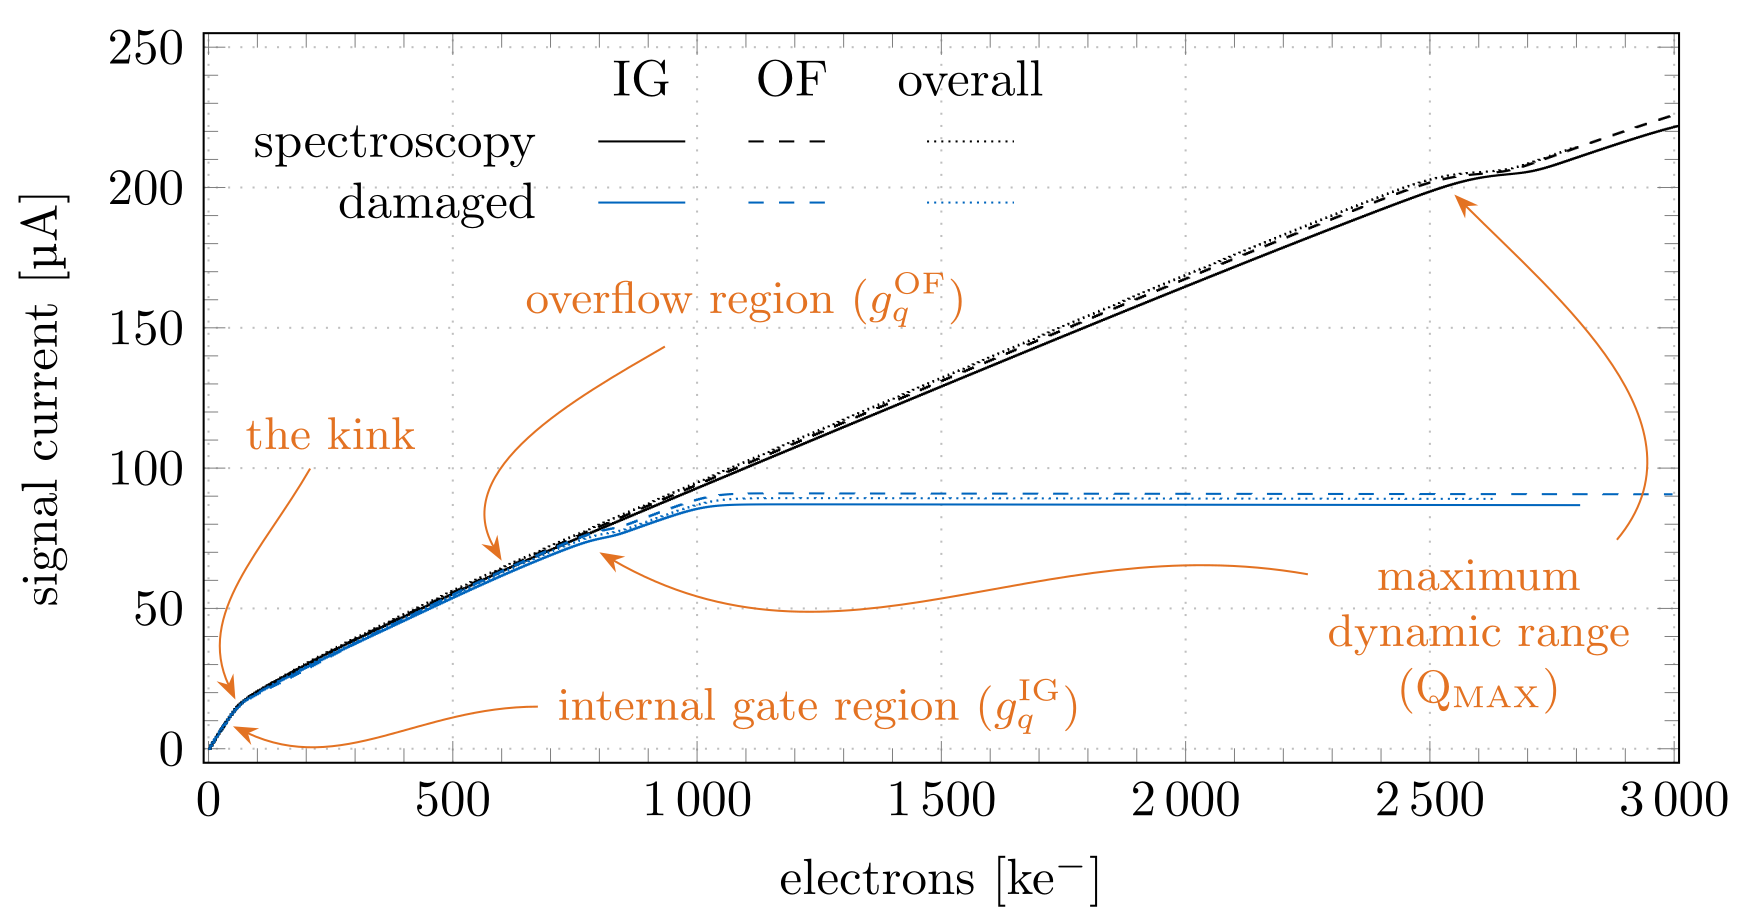
\includegraphics[width=\textwidth]{response.png}
    \end{figure}
    \begin{itemize}
        \item Transfer Gains: $g_q^{IG}=300pA/e^-$;  $g_q^{OF}=~70pA/e^-$ ?
        \item $\approx14e^-$ ENC? [Chap 5.3] $\rightarrow$ 5 nA RMS noise @ drain?
    \end{itemize}
\end{frame}

\begin{frame}
    \frametitle{Column Parallel ADC Specs}
    \begin{itemize}
    \item $P$ power consumption ($\mu W$)
    \item $T_c$ conversion time ($ns$), $T_c=\frac{1}{f_s}$
    \item $A$ silicon area ($\mu m^2$)
    \item $DR$ dynamic range: ratio of max signal to noise floor
    \end{itemize}
    \begin{figure}
        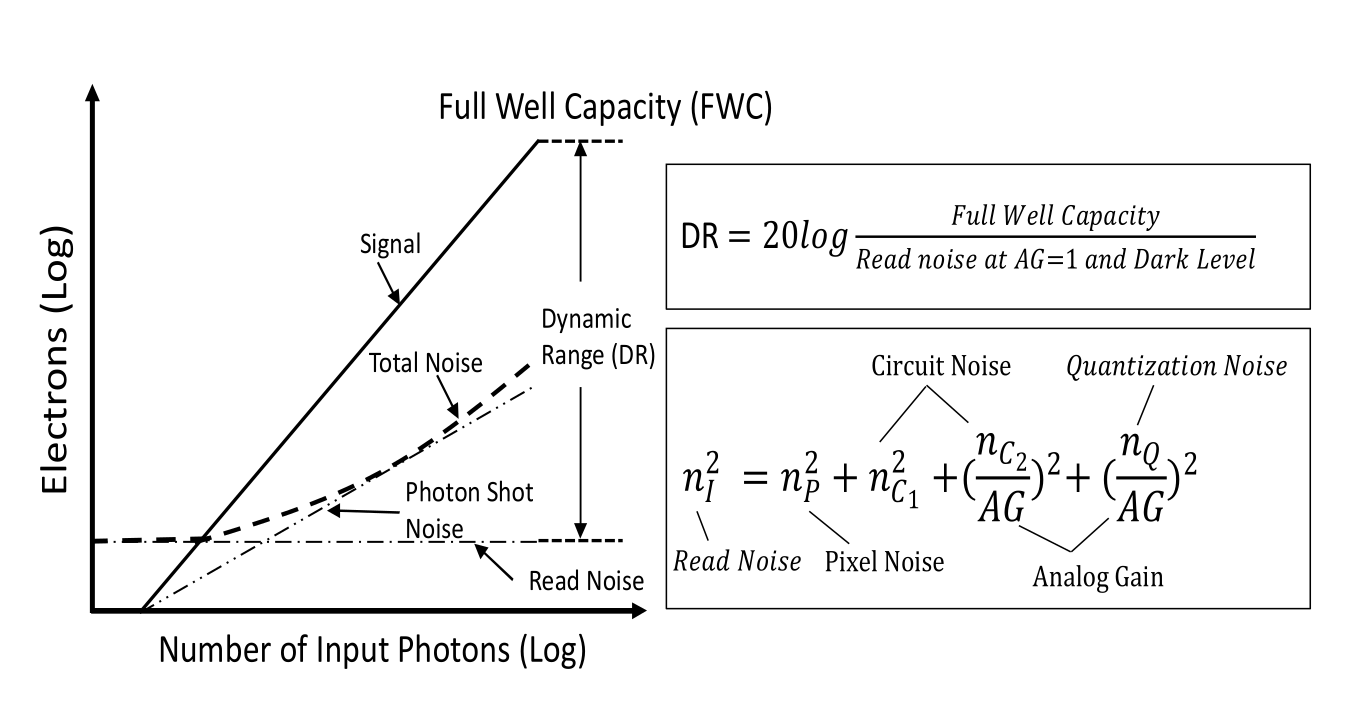
\includegraphics[width=\textwidth]{dr.png}
        \caption{Kwon 2018 ISCAS}
    \end{figure}
\end{frame}

\begin{frame}
    \frametitle{DCD Specs [Peric 2017]}
    \begin{itemize}
    \item $P \approx 5000 \mu W$ consumption per channel
    \item $T_c \approx 100 ns$, no CDS, not fully reserved for ADC
    \item $A = 180\mu m\times 200\mu m = 36000\mu m^2$ silicon area
    \item $1000ke^-$ signal $\rightarrow \Delta 90\mu A$ [Prinker 2022 Chap 6]
    \item 8-bit across DR $\approx 40 LSB$ for first $100ke^-$ signal, $LSB=2500e^-$
    \item $\frac{LSB}{\sqrt{12}} \approx 720 e^-$ quantization error (QE)
    \item $DR = 20\log{(\frac{1000ke^-}{2500e^-})}\approx 48 dB$ best case
    \item ADC non-linearity/skipped codes degrade this even further
    \item Dispersion, leakage, etc not sufficiently corrected by 2-bit pedestal DAC
    \end{itemize}
\end{frame}

\begin{frame}
    \frametitle{Column Parallel ADC Specs [Kwon 2018 ISCAS]}
    \begin{itemize}
        \item $FOM=\frac{P\times T_c \times A}{10^(\frac{DR-1.76}{10})}\bigr[\frac{fJ \cdot \mu m^2 }{conv.step}\bigl]$
        % (5000*100*36000)/(10**((48-1.76)/10))    >>>> 427831
        \item $FOM_{DCD}\approx40000fJ \cdot \mu m^2$
        \item $Rate_{DCD}=10Mpixels/sec$
    \end{itemize}
    \begin{figure}
        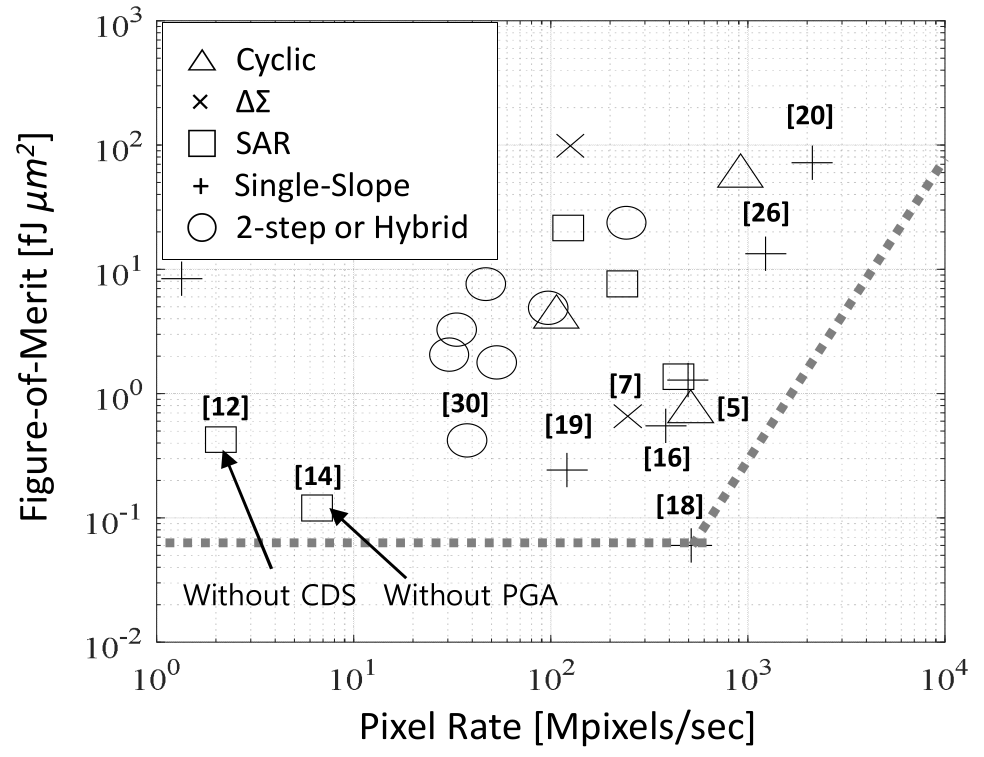
\includegraphics[width=0.6\textwidth]{fom.png}
    \end{figure}
\end{frame}

\begin{frame}
    \frametitle{Data Conversion Summary}
    \begin{itemize}
    \item Pixel Rate ($10Mpixels/sec$) and Area ($36000\mu m^2$) are typical, and sufficient for application
    \item Nominal resolution (8-bit) nowhere near noise limit (QE limited), but acceptable for application ($LSB=2500e^-$)
    \item Nonlinearity + offset significantly degrade beyond nominal resolution
    \item Power consumption of $\approx 5 mW$ seems to offer room for improvement
    \item Need equivalent circuit for drain current signal dynamics
    \end{itemize}
\end{frame}

% \begin{frame}
%     \frametitle{ADC archs}
%     \begin{itemize}
%     \item What ADC archs to try? Cyclic, SAR? (Show diagrams)
%     \item Correlated double sampling could be nice (can we afford the time)
%     \item What if we use a pipeline to digitize after integrating
%     \item Parameters of ASM drain output current (noise, rise/fall times, parasitics)?
%     \item Range of possible hit dynamic range.
%     \end{itemize}
% \end{frame}

\begin{frame}
    \frametitle{Memory Buffer, PLL, Wireline PHY}
    \begin{itemize}
    \item PLL frequency upgrade to 3+ Gbps
    \item SRAM 65nm $0.680\mu m^2$ $\rightarrow$ 28nm $0.127\mu m^2$
    \item SP/DP SRAM vs FIFO?
    \item What speeds are supported by receiver in FPGA?
    \end{itemize}
\end{frame}

\begin{frame}
    \frametitle{Potential architectures}
    \begin{figure}
    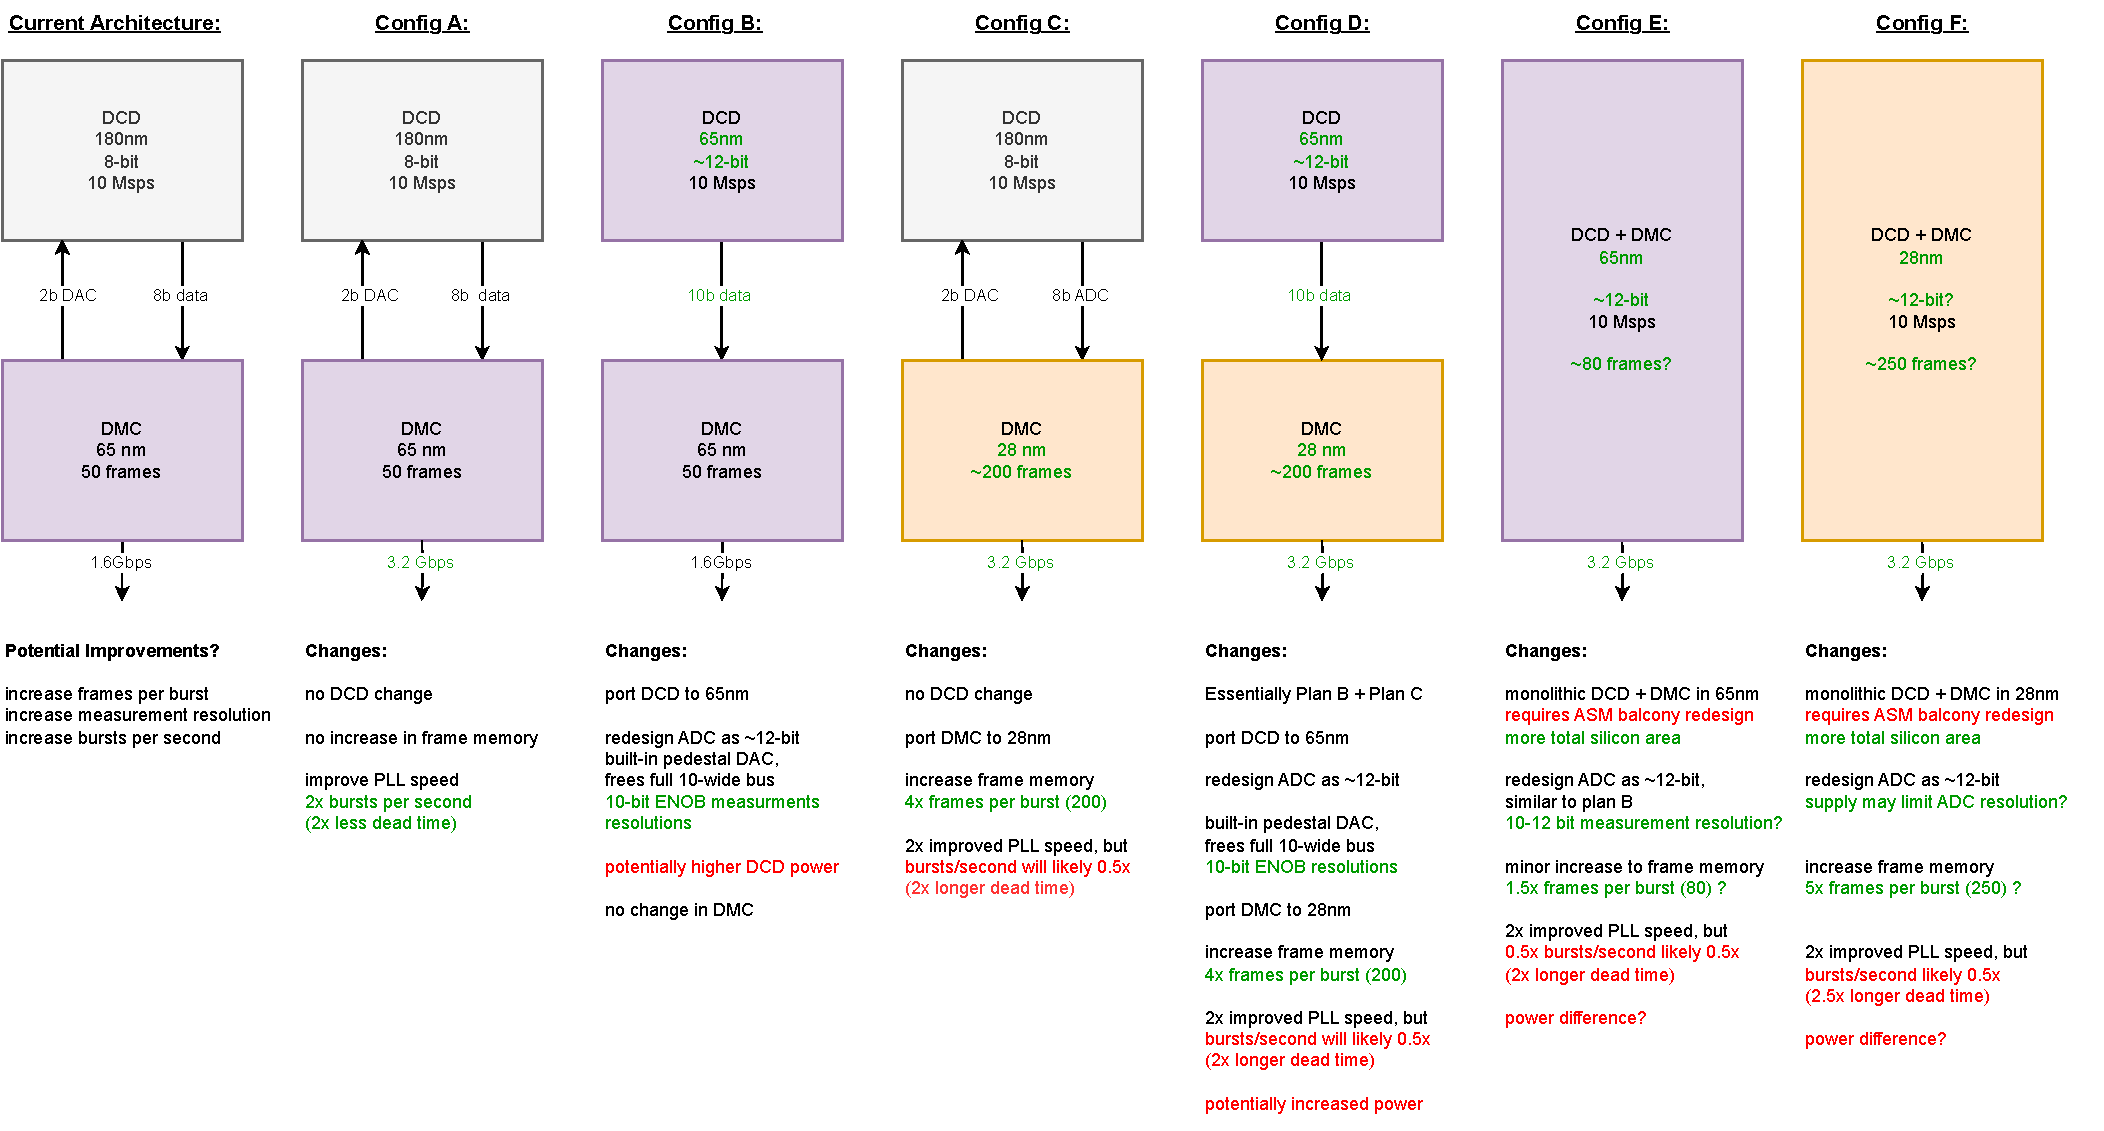
\includegraphics[width=\textwidth]{edet_architectures.drawio.pdf}
    \end{figure}
\end{frame}

\end{document}